% !TEX root = ../main.tex
\chapter{Solution}
\label{chap:solution}

Even though the changes introduced to Rust on \fref{subsec:rfc2000} add the
necessary syntax to abstract code over constant expressions, Rust lacks of a
mechanism reason deeply about constant expressions, and as a consequence is not
possible to typecheck or provide any compile time guarantees over the safety of
using generics over constant values.  On this chapter, we introduce
\textsc{sire}, a symbolic evaluator for Rust, this provides a foundation to
treat function equality via an SMT solver. 

Symbolic execution evaluates a program in an abstract manner, taking symbols
representing each program's input, instead of concrete values, and then
executing the program propagating each symbol. With a symbolic representation
of a function is possible to reason deeply about its behaviour, in particular
is possible to decide if two functions evaluate to the same values for every
possible input or which input for a function would produce a particular result.

With this taken into account, is possible to extend Rust's compiler to reason
about generic types over constant values in a similar manner to its generics
over types counterpart, providing type checking, trait resolution and type
inference for this new kind of generics.

The remaining part of this section explains the inner processes done by
\textsc{sir} and proposes a solution to the problems stated in
\fref{chap:motivation}.

\section{Symbolic execution of Rust programs}
\label{sec:symbolic_execution}

\textsc{sire} is a symbolic executor for the \textsc{mir} of Rust, which is
able to interact with the Rust's compiler. After the compiler generates the
\textsc{mir} for a function, \textsc{sire} takes this representation and
evaluates it into an small symbolic intermediate representation or \textsc{sir}
for short.

Currently \textsc{sire} can only evaluate an small subset of all possible
\textsc{mir} functions. Specifically, it can evaluate functions without mutable
arguments nor mutable references as arguments containing the following subset
of \textsc{mir}:

\begin{itemize}
    \item Statements: \inrust{Assign}, \inrust{StorageLive} and \inrust{StorageDead}.
    \item Terminators: \inrust{Goto}, \inrust{Return}, \inrust{Call} and \inrust{SwitchInt}.
    \item Rvalues: \inrust{BinaryOp}, \inrust{Ref} and \inrust{Use}.
    \item Operands: \inrust{Move}, \inrust{Copy} and \inrust{Constant}.
\end{itemize}

In addition, \textsc{sire} only supports integer and boolean types. Support for
structures, tuples, enumerations and arrays is planned in the future. Floating
point types are not supported given that they lack of the structural equality
property. \footnote{This was stated on
\href{https://github.com/rust-lang/rfcs/blob/master/text/1445-restrict-constants-in-patterns.md}{RFC-1445}.}

\textsc{sire} has an store to read and write symbolic expressions during
evaluation. The symbolic execution of a function starts by allocating each of
the function's arguments as symbols into its store, then each \textsc{mir}
expression is evaluated into a \textsc{sir} expression. When the return
statement of the \textsc{mir} of the function is reached, \textsc{sire} takes
the symbolic expression corresponding to the return value of the function from
its store and returns it, providing a symbolic representation of the function. 


\subsection{Symbolic intermediate representation}

\textsc{sir} is a relatively simple language. Functions are the main construct
of \textsc{sir} and function arguments are numbered following the same
convention as \textsc{mir} where the zeroth argument is the return place. The
grammar for \textsc{sir} can be found on \fref{lst:sir_grammar}.

The body of each function is composed of expressions which can be function
applications, binary operations, switch statements or pure values. 

There are only three kinds of values: Function arguments, constants and
function names. Constants are stored as raw bits with its corresponding type. 

Finally, switch statements are composed by the value to be compared, the
possible values that it can take, and the result for each possible value (there
must be always a default result). 

The evaluation done by \textsc{sire} for each one of the \textsc{mir}
expressions mentioned on section \fref{sec:symbolic_execution} is explained
on \fref{tab:sire_table}.

\begin{table}[ht]
    \centering
    \begin{tabular}{ | c | c | c | }
    \end{tabular}
    \caption{Evaluation of each \textsc{mir} expression, showing the action
    done over the store by \textsc{sire}, and the output \textsc{sir}
    expression. }
  \label{tab:sire_table}
\end{table}


As an example, when executing the code on \fref{lst:rust_sire_example}, the
\textsc{mir} and \textsc{sir} generated can be found on
\fref{lst:mir_sire_example} and \ref{lst:sir_sire_example} respectively. Even
though the code on \fref{lst:rust_sire_example} is similar to the one found in
\fref{lst:sir_sire_example}, \textsc{sire} is executing each instruction of
\fref{lst:mir_sire_example} to generate this representation.

\begin{listing}[ht]
    \begin{minted}{ebnf}
    defun   = '(defun' name {ty} expr ')';
    expr    = value | '('expr {expr}')' | '('op expr expr')' | 
             '(switch' expr {'('expr '->' expr')'} defcase);
    value   = '_'num | '(const' ty num')' | name;
    defcase = '(else ->' expr')';
    ty      = '(int' num')' | '(uint' num')' | 'bool';
    num     = ? a positive integer ?;
    name    = ? an string denoting the name of a function ?;
    op      = ? a binary operator ?;
    \end{minted}
    \caption{\textsc{sir}'s grammar in EBNF}
  \label{lst:sir_grammar}
\end{listing}

\begin{listing}[ht]
    \begin{minted}{rust}
    fn distance(x: i32, y: i32) -> i32 {
        if x > y {
           x - y
        } else {
           y - x
        }
    }
    \end{minted}
    \caption{A simple Rust function to be evaluated using \textsc{sire}}
  \label{lst:rust_sire_example}
\end{listing}

\begin{figure}[ht]
    \centering
    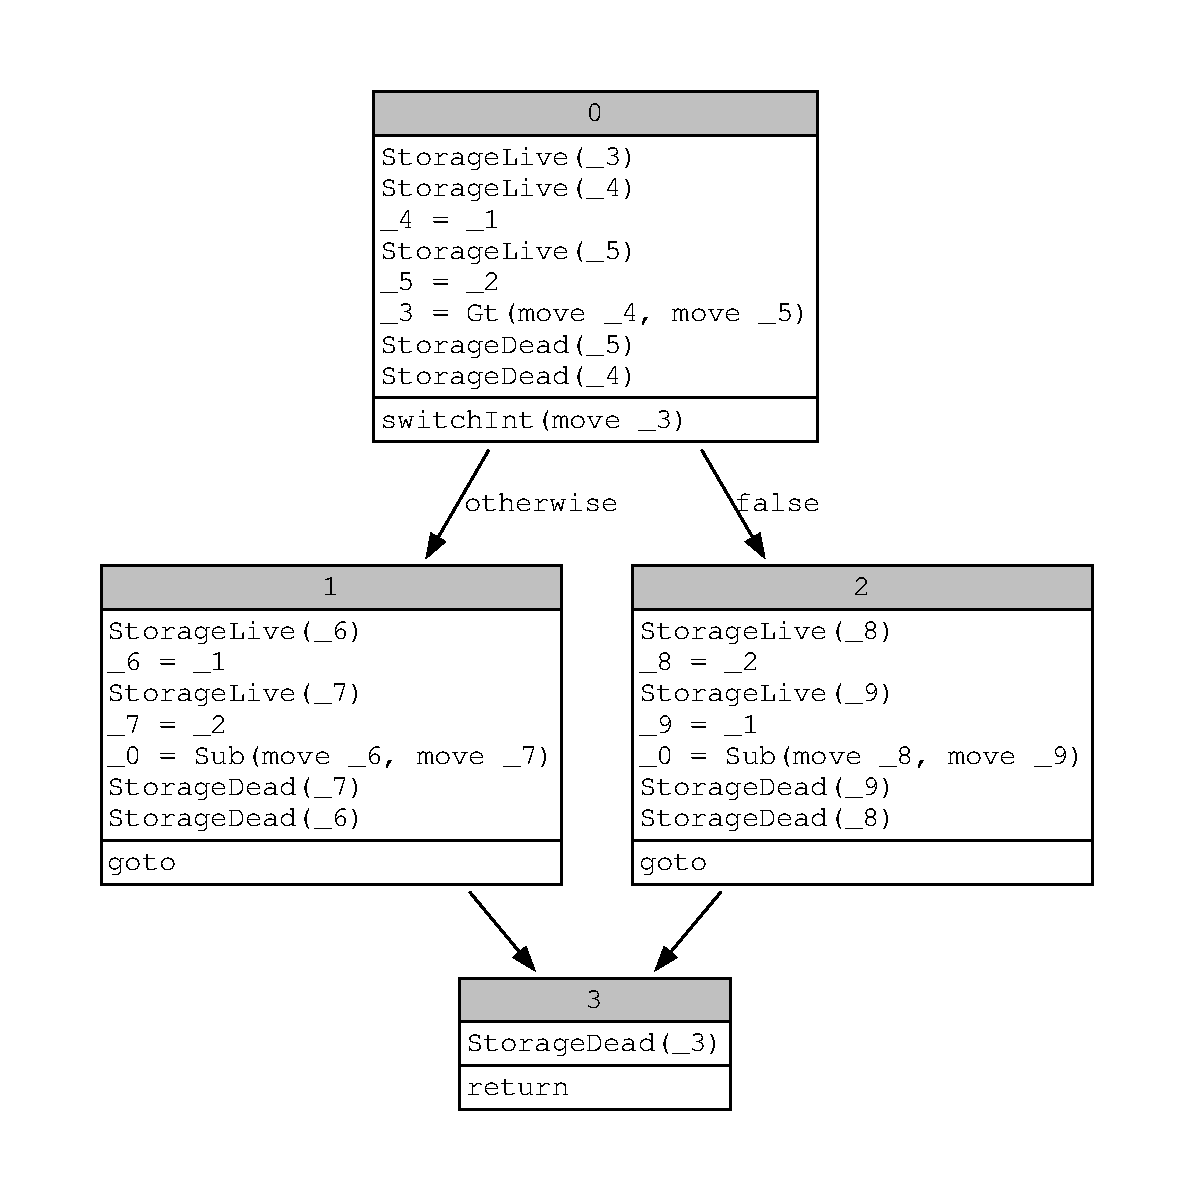
\includegraphics[height=12cm]{images/distance.pdf}
    \caption{The \textsc{mir} of the \inrust{distance} function on \fref{lst:rust_sire_example}}
  \label{lst:mir_sire_example}
\end{figure}

\begin{listing}[ht]
    \begin{minted}{lisp}
    (defun distance (int 32) (int 32) (int 32) 
        (switch (> _1 _2) 
            ((const bool 0) -> (- _2 _1)) 
             (else -> (- _1 _2))))
    \end{minted}
    \caption{The \textsc{sir} of the \inrust{distance} function on \fref{lst:rust_sire_example}}
  \label{lst:sir_sire_example}
\end{listing}

\begin{listing}[ht]
    \begin{minted}{lisp}
    (define-fun distance 
     ((x1 (_ BitVec 32)) (x2 (_ BitVec 32))) (_ BitVec 32) 
     (ite (bvsgt x1 x2) (bvsub x1 x2) (bvsub x2 x1)))
    \end{minted}
    \caption{The \textsc{smt-lib} snippet for the \textsc{sir} of the \inrust{distance} function on \fref{lst:rust_sire_example}}
  \label{lst:smt_sire_example}
\end{listing}


\subsection{Equality of symbolic functions}

Two \textsc{sir} functions are considered equal if they have the same type and
evaluate to the same expression for every possible argument. For simple
arithmetic expressions, this could be achieved via E-unification. However,
\textsc{sir} functions contain control flow operations and recursive calls, in
this case a theorem prover such as Z3 is up to the task. \textsc{sire} can
transform every \textsc{sir} function into an small snippet in the
\textsc{smt-lib} format to use it in an SMT solver.

Integer types on \textsc{sir} are transformed into \textsc{smt-lib} bit vectors
of the corresponding length and the signed or unsigned arithmetic operations
are transformed according to the type of the operands. Switch expressions are
transformed into nested conditionals, preserving the order of the switch
expression's branches. An example of such snippets can be found on
\fref{lst:smt_sire_example}. 

To decide if two functions are equal, is enough to write an small
\textsc{smt-lib} snippet checking if the two functions are equal in their whole
range. On \fref{lst:func_equality}, the \inrust{distance} function is compared
with an alternative implementation found on \fref{lst:alt_distance}. 

\begin{listing}[ht]
    \begin{minted}{rust}
    fn alt_dist(x: i32, y: i32) -> i32 {
        let sign: i32; 
        if x > y {
           sign = 1;
        } else {
           sign = -1;
        }
        sign * (x - y)
    }
    \end{minted}
    \caption{An alternative implementation of the \inrust{distance} function on \fref{lst:rust_sire_example}}
  \label{lst:alt_distance}
\end{listing}

\begin{listing}[ht]
    \begin{minted}{lisp}
    ;; Definition of distance provided by sire
    (define-fun distance 
     ((x1 (_ BitVec 32)) (x2 (_ BitVec 32))) (_ BitVec 32) 
     (ite (bvsgt x1 x2) (bvsub x1 x2) (bvsub x2 x1)))

    ;; Definition of alt_dist provided by sire
    (define-fun alt_dist 
     ((x1 (_ BitVec 32)) (x2 (_ BitVec 32))) (_ BitVec 32) 
     (ite (bvsgt x1 x2) 
      (bvmul (_ bv1 32) (bvsub x1 x2)) 
      (bvmul (_ bv4294967295 32) (bvsub x1 x2))))
    
    ;; Assert that the functions are equal
    (assert (forall ((x1 (_ BitVec 32)) (x2 (_ BitVec 32))) 
     (= (distance x1 x2) (alt_dist x1 x2)))) 

    ;; Check if the assertions can be satisfied
    (check-sat) ; sat
    \end{minted}
    \caption{equality check between the \inrust{distance} and \inrust{alt_dist} functions}
  \label{lst:func_equality}
\end{listing}

It is important to consider that the SMT solver might find no answer to one of
this queries. As a consequence, is not possible to do typechecking or type
inference for every program with generics over constant values.

\section{Typechecking of generics over constants}

\section{Generic traits over constants}

The RFC-2000 allows the user to write implementations for traits which are
generic over constant values, solving the problem of implementing traits for
arrays of arbitrary size as shown in \fref{lst:trait_const_generics}. However,
there is no mechanism to extend trait specialization for generics over constant
values. As a consequence, if a trait has several implementation as in
\fref{lst:trait_const_generics_non_empty} and
\ref{lst:trait_const_generics_empty} is necessary to decide which
implementation will be used on each case. 

The basic strategy to decide which implementation to use is based on the notion
of specificity: If two implementations are overlapping, the compiler will give
priority to the one which is more specific.

On the context of constant expresions, this means that an implementation
without generics over constants is more specific than an implementation with
bounded generics over constants. At the same time, an implementation with
bounded generics over constants is more specific than one without bounds.

When two implementations are generic over constants and have bounds, the
specificity degree will be decided by the specificity of its bounds. If is
possible to proof that one bound implies the other, the first is more specific.

\begin{listing}[ht]
	\begin{minted}{rust}
    impl<A: Sized, B, const N: usize> PartialEq<[B; N]> 
    for [A; N] where A: PartialEq<B> {
        fn eq(&self, other: &[B; N]) -> bool {
            self[..] == other[..]
        }
        fn ne(&self, other: &[B; N]) -> bool {
            self[..] != other[..]
        }
    }
	\end{minted}
    \caption{Implementing the \inrust{PartialEq} trait for all array sizes}
  \label{lst:trait_const_generics}
\end{listing}

\begin{listing}[ht]
	\begin{minted}{rust}
    impl<A: Sized, B, const N: usize> PartialEq<[B; N]> 
    for [A; N] where A: PartialEq<B> with {N > 0} {
        fn eq(&self, other: &[B; N]) -> bool {
            self[..] == other[..]
        }
        fn ne(&self, other: &[B; N]) -> bool {
            self[..] != other[..]
        }
    }
	\end{minted}
    \caption{Implementing the \inrust{PartialEq} trait for non-empty arrays}
  \label{lst:trait_const_generics_non_empty}
\end{listing}

\begin{listing}[ht]
	\begin{minted}{rust}
    impl<A: Sized, B> PartialEq<[B; 0]> 
    for [A; 0] where A: PartialEq<B> {
        fn eq(&self, other: &[B; 0]) -> bool {
            true
        }
        fn ne(&self, other: &[B; 0]) -> bool {
            false
        }
    }
	\end{minted}
    \caption{Implementing the \inrust{PartialEq} trait for empty arrays}
  \label{lst:trait_const_generics_empty}
\end{listing}

\section{Bounds for generics over constants}

\begin{listing}[ht]
	\begin{minted}{rust}
    fn head<T, const N: usize>(array: &[T; N]) -> &T
    where {N > 0} {
        &array[0]
    }
    \end{minted}
    \caption{Type-safe access to the first element of an array without using
    \inrust{Option<T>}}
  \label{lst:head_const_generics}
\end{listing}
